To compare the emanations between desktops, laptops, and an embedded device (an FPGA-based processor), we measured the EM side-channel energy among the 11 instructions given in Table~\ref{insts} for the Lenovo X61 laptop and Dell Optiplex 7010 desktop, and among the 9 instructions in Table~\ref{nios_insts} on the DE1 NIOS FPGA using the 4cm wide square loop probe at the positions shown in Figure~\ref{small_setup}. Each measurement results in a $11 \times 11$ table ($9 \times 9$ table for NIOS) of pairwise A/B SAVAT values for a particular system, with each measurement repeated 10 times over a period of multiple days to assess the impact of changes in radio signal interference, room temperature, errors in positioning the antenna, etc. We include all cases where the A instruction is the same as the B instruction, and these cases are again expected to have a negligible signal at the alternation frequency. The DE1 NIOS FPGA results are given in Table~\ref{fig:FPGA}, the Lenovo X61 laptop results are given in Table~\ref{fig:laptop}, and Dell Optiplex 7010 desktop results are given in Table~\ref{fig:desktop}. All these results were measured at an $80~{\rm kHz}$ alternation frequency, placing the loop probe $10~{\rm cm}$ above each processor as shown in Figure~\ref{small_setup}. 

The power spectrum is measured at the same alternation frequency of $1/T=80~{\rm kHz}$, to quantify the EM side-channel signal created by the difference between the A and B instructions. A comparison of recorded spectra produced by alternating between an off-chip memory load vs. an on-chip cache load (LDM/LDL1) instruction executing on a Cyclone II FPGA, a Lenovo X61 Laptop, and a Dell Optiplex 7010 Desktop is shown in Figure~\ref{LDM-LDL1-Spectrum}. We can be confident the signals we observe are not due to other unrelated signals (such as nearby switching power supplies, CRT or LCD monitors, or other cabling) because the signal is only present when the A and B instructions differ (e.g. there is no signal for LDM/LDM), and because the observed peak follows the intended alternation frequency. 
%other features of the graph
\begin{figure}[htb]
\centering
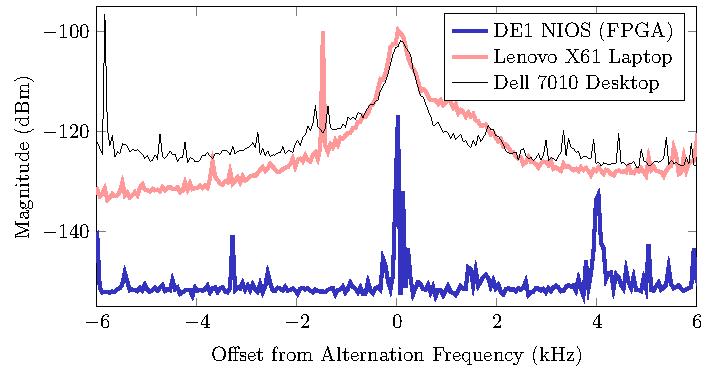
\includegraphics[width=5in]{../emc_comparison_4/spect_cmp.pdf}
\caption{Comparison of power spectra for LDM/LDL1 on DE1 NIOS (FPGA), Lenovo X61 laptop, and Dell 7010 desktop.}
\label{LDM-LDL1-Spectrum}
\end{figure}

It is interesting to observe that the generated signals are almost perfectly concentrated at the intended alternation frequency for the FPGA board, but are much more spread for laptops and desktops. One possible explanation for the wider spectra is that the alternation frequency cannot be controlled perfectly in laptops and desktops and that the alternation period $T$ varies slightly in complex processors, resulting in the dispersion of power around the alternation frequency. This is likely caused by greater variation in the total off-chip memory access time on the desktop and laptop systems. Furthermore, we observe that emanations from desktops and laptops are much stronger than those from FPGA, which aligns with the number of switching transistors and power expended in complex systems. To ensure we are capturing all the power generated by our benchmark, we integrate over the frequency band from $2.5~{\rm kHz}$ below to $2.5~{\rm kHz}$ above the alternation frequency to find the total generated signal power. This power is converted to energy per instruction (SAVAT) according to Equation~\ref{eqn:meas_ese}. 

\begin{table}[htb]
  \scriptsize
  \setlength{\tabcolsep}{2.3pt}
  \setlength\extrarowheight{1pt}
  \caption{SAVAT collected $10~{\rm cm}$ above the NIOS processor on the DE1 FPGA board with the 4cm coil probe. Values are in zepto-Joules.}
  \begin{tabu}{|c||c|c|c|c|c|c|c|c|c|} \hline
    & \textbf{LDM} & \textbf{STM} & \textbf{LDL1} & \textbf{STL1} & \textbf{NOI} & \textbf{ADD} & \textbf{SUB} & \textbf{MUL} & \textbf{DIV}
    \\ \hhline{|=||=|=|=|=|=|=|=|=|=|}
    \textbf{LDM} &  {0.05} &  {1.84} &  {3.77} &  {4.13} &  {4.90} &  {6.22} &  {7.22} &  {3.98} &  {4.02} \\ \hline
    \textbf{STM} &  {1.74} &  {0.03} &  {1.34} &  {1.15} &  {1.33} &  {1.35} &  {1.59} &  {1.31} &  {1.38} \\ \hline
    \textbf{LDL1} &  {3.93} &  {1.47} &  {0.03} &  {0.18} &  {0.66} &  {0.74} &  {1.18} &  {0.05} &  {0.04} \\ \hline
    \textbf{STL1} &  {4.32} &  {1.23} &  {0.20} &  {0.01} &  {0.24} &  {0.22} &  {0.46} &  {0.10} &  {0.24} \\ \hline
    \textbf{NOI} &  {5.11} &  {1.42} &  {0.70} &  {0.26} &  {0.02} &  {0.02} &  {0.07} &  {0.53} &  {0.87} \\ \hline
    \textbf{ADD} &  {5.11} &  {1.40} &  {0.83} &  {0.26} &  {0.02} &  {0.02} &  {0.03} &  {0.68} &  {0.87} \\ \hline
    \textbf{SUB} &  {7.03} &  {1.60} &  {1.05} &  {0.45} &  {0.05} &  {0.07} &  {0.02} &  {1.03} &  {1.25} \\ \hline
    \textbf{MUL} &  {4.10} &  {1.44} &  {0.04} &  {0.09} &  {0.55} &  {0.63} &  {0.95} &  {0.00} &  {0.08} \\ \hline
    \textbf{DIV} &  {4.28} &  {1.54} &  {0.05} &  {0.24} &  {0.91} &  {0.92} &  {1.29} &  {0.08} &  {0.02} \\ \hline

     \end{tabu}

  \label{fig:FPGA}
\end{table}

\begin{table}[htb]
  \scriptsize
  \setlength{\tabcolsep}{2.3pt}
  \setlength\extrarowheight{1pt}
  \caption{SAVAT collected $10~{\rm cm}$ above the Lenovo X61 laptop  with the 4cm coil probe. Values are in zepto-Joules.}
  \begin{tabu}{|c||c|c|c|c|c|c|c|c|c|c|c|} \hline
    & \textbf{LDM} & \textbf{STM} & \textbf{LDL2} & \textbf{STL2} & \textbf{LDL1} & \textbf{STL1} & \textbf{NOI} & \textbf{ADD} & \textbf{SUB} & \textbf{MUL} & \textbf{DIV}
    \\ \hhline{|=||=|=|=|=|=|=|=|=|=|=|=|}
    \textbf{LDM} & {0} & {35} & {182} & {96} & {610} & {661} & {515} & {667} & {659} & {661} & {2160} \\ \hline
    \textbf{STM} & {45} & {0} & {6} & {6} & {21} & {24} & {13} & {18} & {18} & {18} & {130} \\ \hline
    \textbf{LDL2} & {175} & {6} & {0} & {18} & {176} & {195} & {163} & {203} & {200} & {203} & {283} \\ \hline
    \textbf{STL2} & {96} & {11} & {16} & {0} & {263} & {292} & {256} & {301} & {292} & {297} & {363} \\ \hline
    \textbf{LDL1} & {637} & {23} & {191} & {298} & {0} & {0} & {0} & {0} & {0} & {0} & {19} \\ \hline
    \textbf{STL1} & {667} & {45} & {185} & {302} & {0} & {0} & {0} & {0} & {0} & {0} & {15} \\ \hline
    \textbf{NOI} & {536} & {13} & {161} & {262} & {0} & {0} & {0} & {0} & {0} & {0} & {14} \\ \hline
    \textbf{ADD} & {676} & {37} & {193} & {312} & {1} & {0} & {0} & {0} & {0} & {1} & {13} \\ \hline
    \textbf{SUB} & {668} & {23} & {190} & {307} & {1} & {0} & {0} & {0} & {0} & {0} & {18} \\ \hline
    \textbf{MUL} & {677} & {29} & {198} & {310} & {1} & {0} & {0} & {0} & {0} & {0} & {14} \\ \hline
    \textbf{DIV} & {2224} & {176} & {275} & {363} & {19} & {16} &  {14} & {13} & {15} & {14} & {2} \\ \hline
  \end{tabu}

  \label{fig:laptop}
\end{table}


\begin{table}[htb]
  \scriptsize
  \setlength{\tabcolsep}{2.3pt}
  \setlength\extrarowheight{1pt}
  \caption{SAVAT collected $10~{\rm cm}$ above the Dell 7010 desktop with the 4cm coil probe. Values are in zepto-Joules.}
  \begin{tabu}{|c||c|c|c|c|c|c|c|c|c|c|c|} \hline
    & \textbf{LDM} & \textbf{STM} & \textbf{LDL2} & \textbf{STL2} & \textbf{LDL1} & \textbf{STL1} & \textbf{NOI} & \textbf{ADD} & \textbf{SUB} & \textbf{MUL} & \textbf{DIV}
    \\ \hhline{|=||=|=|=|=|=|=|=|=|=|=|=|}
    \textbf{LDM} &  {2} &  {262} &  {84} &  {82} &  {140} &  {170} &  {155} &  {179} &  {196} &  {148} &  {861} \\ \hline
    \textbf{STM} &  {55} &  {1} &  {164} &  {162} &  {306} &  {334} &  {369} &  {420} &  {418} &  {318} &  {1490} \\ \hline
    \textbf{LDL2} &  {85} &  {153} &  {1} &  {1} &  {32} &  {43} &  {43} &  {51} &  {55} &  {42} &  {297} \\ \hline
    \textbf{STL2} &  {84} &  {165} &  {2} &  {1} &  {46} &  {44} &  {85} &  {72} &  {66} &  {33} &  {256} \\ \hline
    \textbf{LDL1} &  {140} &  {296} &  {27} &  {24} &  {0} &  {1} &  {2} &  {3} &  {5} &  {1} &  {108} \\ \hline
    \textbf{STL1} &  {143} &  {321} &  {29} &  {44} &  {0} &  {0} &  {5} &  {4} &  {3} &  {1} &  {61} \\ \hline
    \textbf{NOI} &  {144} &  {332} &  {44} &  {39} &  {2} &  {0} &  {0} &  {0} &  {0} &  {0} &  {76} \\ \hline
    \textbf{ADD} &  {198} &  {423} &  {58} &  {54} &  {5} &  {1} &  {1} &  {1} &  {1} &  {1} &  {60} \\ \hline
    \textbf{SUB} &  {145} &  {321} &  {38} &  {55} &  {1} &  {1} &  {2} &  {1} &  {2} &  {2} &  {48} \\ \hline
    \textbf{MUL} &  {189} &  {431} &  {64} &  {49} &  {7} &  {1} &  {1} &  {2} &  {2} &  {2} &  {59} \\ \hline
    \textbf{DIV} &  {708} &  {1400} &  {193} &  {246} &  {58} &  {56} &  {25} &  {70} &  {31} &  {76} &  {2} \\ \hline

  \end{tabu}
  \label{fig:desktop}
   \end{table}

These tables only describe one possible probe position and orientation, though there are several trends that have been found to be generally consistent across many probe positions and across the tested systems. First, the differences between the ADD, SUB and NOI columns (and rows) is generally within experimental error. This means that adding (or removing) a single integer add or subtract instruction, or substituting an ADD for a SUB has an extremely small impact on emanations. Second, the integer divide instruction generates significantly more SAVAT than the add and subtract operation. This is likely because division is a more complex operation executed over several clock cycles, expending more energy. Finally, regarding loads and stores, more side channel energy per instruction is available to the attacker as higher levels of the memory hierarchy are accessed. In other words, generally L2 cache accesses have higher SAVAT than L1 cache accesses, and memory accesses have higher SAVAT than L1 and L2 cache accesses. This is consistent with the intuition that higher levels of the memory heirarchy should emanate more strongly since such accesses {\it expend} more energy per instruction, activating more circuitry and drawing more current through longer wires (antennas). %Finally, the SAVAT values are in line with the power levels of the processor and system: the FPGA uses less than 2 Watts while the laptop and desktop use greater than 50 Watts, which is consistent with the lower FPGA SAVAT values. 
